\documentclass[a4paper,12pt]{article}

\usepackage[top=25mm, left=25mm, right=25mm, bottom=25mm, total={175mm, 247mm}, includehead=false, includefoot=false]{geometry}
\usepackage{multicol}
\usepackage{colortbl}
\usepackage{hyperref}
\usepackage{graphicx}
\usepackage{subcaption}

\usepackage{parskip}
\setlength{\parskip}{\medskipamount}
\makeatletter 
\newcommand{\@minipagerestore}{
\setlength{\parindent}{15pt}
\setlength{\parskip}{\medskipamount}}
\makeatother

\usepackage{Sweave}
\begin{document}
\Sconcordance{concordance:exoplanety.tex:exoplanety.Rnw:%
1 17 1 1 0 26 1 1 162 9 1 1 8 1 2 8 1 1 7 1 2 9 1 1 2 15 0 1 2 2 1 1 2 %
13 0 1 2 6 1 1 2 15 0 1 2 17 1 1 2 15 0 1 2 7 1 1 2 15 0 1 2 19 1 1 2 %
15 0 1 2 2 1 1 2 13 0 1 2 6 1 1 2 15 0 1 2 17 1 1 2 15 0 1 2 7 1 1 2 15 %
0 1 2 18 1 1 2 15 0 1 2 2 1 1 2 13 0 1 2 5 1 1 28 9 1 1 2 15 0 1 2 1 1 %
1 2 15 0 1 2 1 1 1 2 15 0 1 2 3 1 1 2 7 0 1 2 3 1 1 2 27 0 1 2 6 1 1 4 %
5 1 1 2 13 0 1 2 1 1 1 5 13 0 1 2 2 1 1 2 7 0 1 2 5 1 1 2 7 0 1 2 6 1 1 %
8 13 0 1 2 9 1 1 10 1 2 7 1 1 13 1 2 3 1 1 2 15 0 1 2 9 1 1 10 1 2 10 1 %
1 10 1 2 4 1}



\begin{titlepage}
\begin{center}
\Large \rmfamily
Univerzita Pardubice
\par
Fakulta elektrotechniky a informatiky
\par
\vspace{0pt plus 3fill}
Statistické vyhodnocení objevených exoplanet
\par
\bigskip
\par
Michal Struna
\par
\vspace{0pt plus 5fill}
Semestrální práce
\par
2019
\end{center}
\end{titlepage}
\stepcounter{page}



\section{Úvod}

Tato semestrální práce zkoumá data a~vztahy mezi daty u~objevených exoplanet. Jedná se o~planety mimo sluneční soustavu, kterých bylo k~listopadu 2019 potvrzeno 4104. K~práci byl využit archiv pocházející od NASA a obsahujícící všechny tyto planety. Je dostupný přes webové API nebo ke stažení jako CSV na adrese \url{https://exoplanetarchive.ipac.caltech.edu}.

\section{Zkoumané údaje}
\subsection{Způsob objevení}

\begin{center}

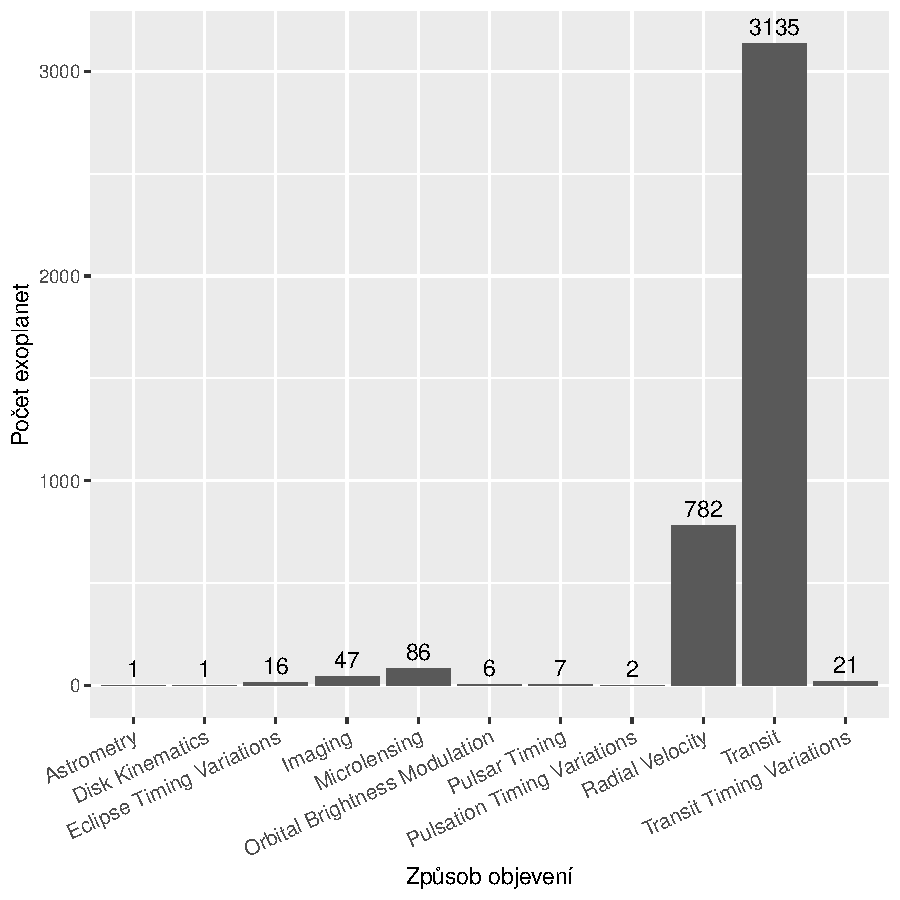
\includegraphics{exoplanety-discmethod}

\end{center}

Protože exoplanety nelze pozorovat přímo, jsou k jejich objevování využívány různé techniky nepřímého pozorování. Počet planet objevených jednotlivými metodami je zobrazen v histogramu výše.

\newpage
\subsection{Poloměr planety}
\begin{figure}[!htb]
\centering
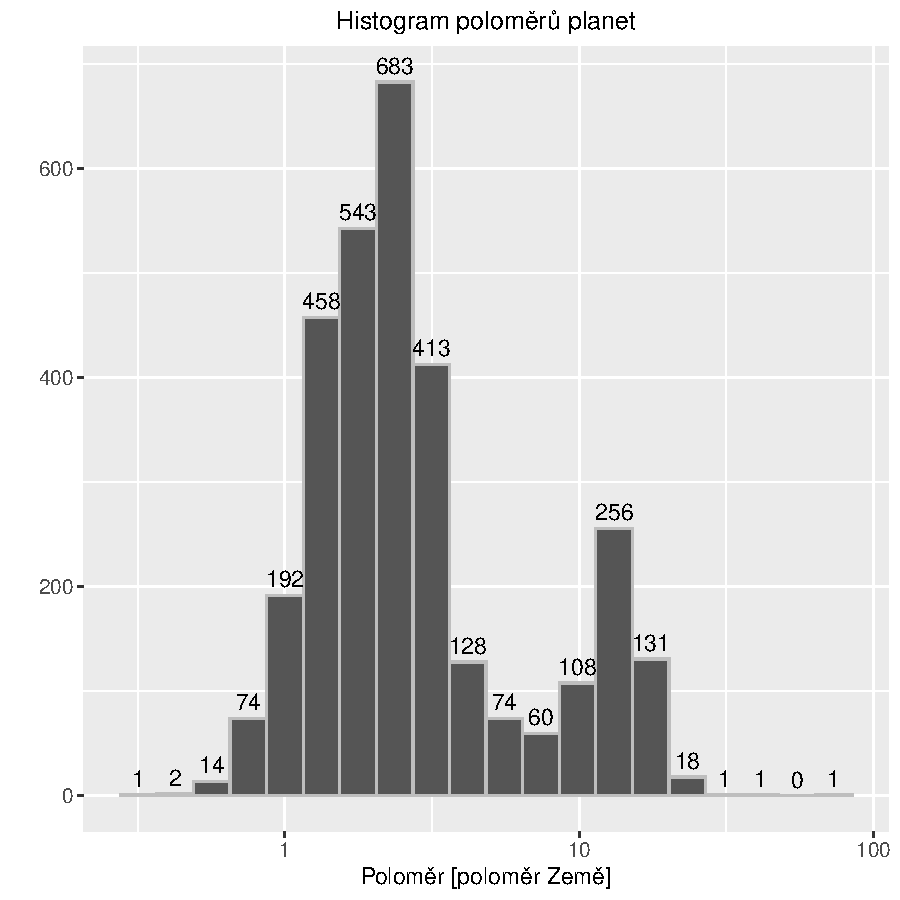
\includegraphics{exoplanety-003}
\end{figure}

\setlength{\columnsep}{0.43\textwidth}
\begin{multicols}{2}
\begin{minipage}{0.7\textwidth}
Poloměr planet je uváděn v poloměrech Země. Histogram četností planet v jednotlivých velikostních kategoriích má tvar bimodálního rozdělení. To je způsobeno tím, že terestrické (kamenné) planety podobné Zemi jsou často mnohem menší, než velcí plynní obři typu Jupiter.

Všechny planety byly následně rozdělěny do všeobecně uznávaných velikostních kategorií dle následující tabulky:
\end{minipage}
\begin{minipage}{0.3\textwidth}
% latex table generated in R 3.5.2 by xtable 1.8-4 package
% Mon Dec  9 22:38:36 2019
\begin{tabular}{| l| l|}
   \hline
{\cellcolor[rgb]{0.85, 0.85, 0.85}{ Min }} & 0.34 \\ 
   \hline
{\cellcolor[rgb]{0.85, 0.85, 0.85}{ Qu1 }} & 1.57 \\ 
   \hline
{\cellcolor[rgb]{0.85, 0.85, 0.85}{ Median }} & 2.34 \\ 
   \hline
{\cellcolor[rgb]{0.85, 0.85, 0.85}{ Mean }} & 4.23 \\ 
   \hline
{\cellcolor[rgb]{0.85, 0.85, 0.85}{ Qu3 }} & 3.60 \\ 
   \hline
{\cellcolor[rgb]{0.85, 0.85, 0.85}{ Max }} & 77.34 \\ 
   \hline
\end{tabular}\end{minipage}
\end{multicols}

% latex table generated in R 3.5.2 by xtable 1.8-4 package
% Mon Dec  9 22:38:36 2019
\begin{table}[ht]
\centering
\begin{tabular}{| l| l| l| l| l|}
  \hline
 & {\cellcolor[rgb]{0.85, 0.85, 0.85}{ Mercurian }} & {\cellcolor[rgb]{0.85, 0.85, 0.85}{ Earth }} & {\cellcolor[rgb]{0.85, 0.85, 0.85}{ Neptunian }} & {\cellcolor[rgb]{0.85, 0.85, 0.85}{ Jovian }} \\ 
  \hline
{\cellcolor[rgb]{0.85, 0.85, 0.85}{ Poloměr [poloměry Země] }} & < 0,7 & 0,7-2 & 2-6 & > 6 \\ 
   \hline
{\cellcolor[rgb]{0.85, 0.85, 0.85}{ Počet }} & {\cellcolor[rgb]{ 0.980959634424981 ,  1 ,  0.980959634424981 }{ 25 }} & {\cellcolor[rgb]{ 0.0677837014470678 ,  1 ,  0.0677837014470678 }{ 1224 }} & {\cellcolor[rgb]{ 0 ,  1 ,  0 }{ 1313 }} & {\cellcolor[rgb]{ 0.546077684691546 ,  1 ,  0.546077684691546 }{ 596 }} \\ 
   \hline
\end{tabular}
\caption{Rozdělení planet do kategorií dle velikosti} 
\end{table}
\newpage
\subsection{Vzdálenost od Země}

\setlength{\columnsep}{0\textwidth}
\begin{multicols}{2}
\begin{minipage}{0.3\textwidth}
% latex table generated in R 3.5.2 by xtable 1.8-4 package
% Mon Dec  9 22:38:36 2019
\begin{tabular}{| l| l|}
   \hline
{\cellcolor[rgb]{0.85, 0.85, 0.85}{ Min }} & 4.24 \\ 
   \hline
{\cellcolor[rgb]{0.85, 0.85, 0.85}{ Qu1 }} & 501.19 \\ 
   \hline
{\cellcolor[rgb]{0.85, 0.85, 0.85}{ Median }} & 1542.21 \\ 
   \hline
{\cellcolor[rgb]{0.85, 0.85, 0.85}{ Mean }} & 2069.64 \\ 
   \hline
{\cellcolor[rgb]{0.85, 0.85, 0.85}{ Qu3 }} & 2816.64 \\ 
   \hline
{\cellcolor[rgb]{0.85, 0.85, 0.85}{ Max }} & 27710.00 \\ 
   \hline
\end{tabular}\end{minipage}
\begin{minipage}{0.7\textwidth}
Vzdálenost planet od Země je udávána ve světelných letech (zkratka ly). Světelný rok je vzdálenost, kterou světlo ve vakuu urazí za jeden rok, tedy přibližně $9.46 * 10^{12}$~km.

Nejbližší exoplaneta vůbec, ve vzdálenosti 4,2~ly od Země, obíhá kolem nejbližší hvězdy Slunci -- Proxima Centauri. Většina planet se ale nachází ve vzdálenosti 1~000 až 3~000~ly.
\end{minipage}
\end{multicols}

\subsection{Hmotnost planety}

\setlength{\columnsep}{0.43\textwidth}
\begin{multicols}{2}
\begin{minipage}{0.7\textwidth}
Hmotnost planet je vyjádřená v hmotnostech Země. Nejvyhledávanějšími planety jsou ty, jejichž hmotnost je podobná Zemi.

Hmotnost malých planet je obtížné určit, a proto je u více jak poloviny (2~448) hmotnost neznámá. Z~tohoto důvodu je 75 \% změřených planet více jak 28krát hmotnějších, než Země.
\end{minipage}
\begin{minipage}{0.3\textwidth}
% latex table generated in R 3.5.2 by xtable 1.8-4 package
% Mon Dec  9 22:38:36 2019
\begin{tabular}{| l| l|}
   \hline
{\cellcolor[rgb]{0.85, 0.85, 0.85}{ Min }} & 0.02 \\ 
   \hline
{\cellcolor[rgb]{0.85, 0.85, 0.85}{ Qu1 }} & 28.38 \\ 
   \hline
{\cellcolor[rgb]{0.85, 0.85, 0.85}{ Median }} & 273.33 \\ 
   \hline
{\cellcolor[rgb]{0.85, 0.85, 0.85}{ Mean }} & 798.17 \\ 
   \hline
{\cellcolor[rgb]{0.85, 0.85, 0.85}{ Qu3 }} & 807.26 \\ 
   \hline
{\cellcolor[rgb]{0.85, 0.85, 0.85}{ Max }} & 17668.17 \\ 
   \hline
\end{tabular}\end{minipage}
\end{multicols}

\subsection{Velká poloosa}

\setlength{\columnsep}{0\textwidth}
\begin{multicols}{2}
\begin{minipage}{0.3\textwidth}
% latex table generated in R 3.5.2 by xtable 1.8-4 package
% Mon Dec  9 22:38:36 2019
\begin{tabular}{| l| l|}
   \hline
{\cellcolor[rgb]{0.85, 0.85, 0.85}{ Min }} & 0.00 \\ 
   \hline
{\cellcolor[rgb]{0.85, 0.85, 0.85}{ Qu1 }} & 0.06 \\ 
   \hline
{\cellcolor[rgb]{0.85, 0.85, 0.85}{ Median }} & 0.12 \\ 
   \hline
{\cellcolor[rgb]{0.85, 0.85, 0.85}{ Mean }} & 6.56 \\ 
   \hline
{\cellcolor[rgb]{0.85, 0.85, 0.85}{ Qu3 }} & 0.69 \\ 
   \hline
{\cellcolor[rgb]{0.85, 0.85, 0.85}{ Max }} & 2500.00 \\ 
   \hline
\end{tabular}\end{minipage}
\begin{minipage}{0.7\textwidth}
Velká poloosa je průměrem minimální a~maximální vzdálenosti planety od své hvězdy. Je udávána v~astronomických jednotkách ~(AU), která je odzvozena od velké poloosy Země (149~597~870 km).

Opět platí, že nejvyhledávanější hodnota je rovna 1, protože pak na planetě budou Zemi podobnější podmínky. Záleží však i~na typu hvězdy.
\end{minipage}
\end{multicols}

\subsection{Perioda oběhu planety}

\setlength{\columnsep}{0.43\textwidth}
\begin{multicols}{2}
\begin{minipage}{0.7\textwidth}
Perioda oběhu planety udává, za kolik pozemských dní planeta oběhne kolem své hvězdy. 75~\% planet má dobu oběhu menší než 42~dní a pouze malé procento planet větší, než 1~000~dní.

Planety byly dále rozděleny do kategorií dle následující tabulky v~závislosti na jejich periodě oběhu:

\end{minipage}

\begin{minipage}{0.3\textwidth}
% latex table generated in R 3.5.2 by xtable 1.8-4 package
% Mon Dec  9 22:38:36 2019
\begin{tabular}{| l| l|}
   \hline
{\cellcolor[rgb]{0.85, 0.85, 0.85}{ Min }} & 0.09 \\ 
   \hline
{\cellcolor[rgb]{0.85, 0.85, 0.85}{ Qu1 }} & 4.49 \\ 
   \hline
{\cellcolor[rgb]{0.85, 0.85, 0.85}{ Median }} & 11.87 \\ 
   \hline
{\cellcolor[rgb]{0.85, 0.85, 0.85}{ Mean }} & 2306.82 \\ 
   \hline
{\cellcolor[rgb]{0.85, 0.85, 0.85}{ Qu3 }} & 42.60 \\ 
   \hline
{\cellcolor[rgb]{0.85, 0.85, 0.85}{ Max }} & 7300000.00 \\ 
   \hline
\end{tabular}\end{minipage}
\end{multicols}

% latex table generated in R 3.5.2 by xtable 1.8-4 package
% Mon Dec  9 22:38:36 2019
\begin{table}[ht]
\centering
\begin{tabular}{| l| l| l| l| l|}
  \hline
 & {\cellcolor[rgb]{0.85, 0.85, 0.85}{ Lava }} & {\cellcolor[rgb]{0.85, 0.85, 0.85}{ Hot }} & {\cellcolor[rgb]{0.85, 0.85, 0.85}{ Normal }} & {\cellcolor[rgb]{0.85, 0.85, 0.85}{ Cold }} \\ 
  \hline
{\cellcolor[rgb]{0.85, 0.85, 0.85}{ Doba oběhu [dny] }} & < 5 & 5-50 & 50-500 & > 500 \\ 
   \hline
{\cellcolor[rgb]{0.85, 0.85, 0.85}{ Počet }} & {\cellcolor[rgb]{ 0.434627170582227 ,  1 ,  0.434627170582227 }{ 1107 }} & {\cellcolor[rgb]{ 0 ,  1 ,  0 }{ 1958 }} & {\cellcolor[rgb]{ 0.724208375893769 ,  1 ,  0.724208375893769 }{ 540 }} & {\cellcolor[rgb]{ 0.805413687436159 ,  1 ,  0.805413687436159 }{ 381 }} \\ 
   \hline
\end{tabular}
\caption{Rozdělení planet do kategorií dle periody oběhu} 
\end{table}
\newpage  
\subsection{Počet planet v systému}

\setlength{\columnsep}{0\textwidth}
\begin{multicols}{2}
\begin{minipage}{0.3\textwidth}
% latex table generated in R 3.5.2 by xtable 1.8-4 package
% Mon Dec  9 22:38:36 2019
\begin{tabular}{| l| l|}
   \hline
{\cellcolor[rgb]{0.85, 0.85, 0.85}{ Min }} & 1.00 \\ 
   \hline
{\cellcolor[rgb]{0.85, 0.85, 0.85}{ Qu1 }} & 1.00 \\ 
   \hline
{\cellcolor[rgb]{0.85, 0.85, 0.85}{ Median }} & 1.00 \\ 
   \hline
{\cellcolor[rgb]{0.85, 0.85, 0.85}{ Mean }} & 1.78 \\ 
   \hline
{\cellcolor[rgb]{0.85, 0.85, 0.85}{ Qu3 }} & 2.00 \\ 
   \hline
{\cellcolor[rgb]{0.85, 0.85, 0.85}{ Max }} & 8.00 \\ 
   \hline
\end{tabular}\end{minipage}
\begin{minipage}{0.7\textwidth}
V~jedné soustavě je zřídkakdy pouze 1~planeta, avšak z~důvodu omezených podmínek pozorování je~i~přesto více jak polovina planet v systému samotných.

Z druhé strany existuje 1~systém se 7~planetami a 1~systém s~8~planetami.
\end{minipage}
\end{multicols}

\subsection{Poloměr hvězdy}

\setlength{\columnsep}{0.43\textwidth}
\begin{multicols}{2}
\begin{minipage}{0.7\textwidth}
Poloměr rodičovských hvězd planet je určován v~poloměrech Slunce.

50~\% objevených planet obíhá kolem hvězdy, jejíž poloměr se pohybuje mezi 0,8~až 1,26~poloměry Slunce.
\end{minipage}
\begin{minipage}{0.3\textwidth}
% latex table generated in R 3.5.2 by xtable 1.8-4 package
% Mon Dec  9 22:38:36 2019
\begin{tabular}{| l| l|}
   \hline
{\cellcolor[rgb]{0.85, 0.85, 0.85}{ Min }} & 0.01 \\ 
   \hline
{\cellcolor[rgb]{0.85, 0.85, 0.85}{ Qu1 }} & 0.80 \\ 
   \hline
{\cellcolor[rgb]{0.85, 0.85, 0.85}{ Median }} & 0.98 \\ 
   \hline
{\cellcolor[rgb]{0.85, 0.85, 0.85}{ Mean }} & 1.54 \\ 
   \hline
{\cellcolor[rgb]{0.85, 0.85, 0.85}{ Qu3 }} & 1.26 \\ 
   \hline
{\cellcolor[rgb]{0.85, 0.85, 0.85}{ Max }} & 71.23 \\ 
   \hline
\end{tabular}\end{minipage}
\end{multicols}

\subsection{Hmotnost hvězdy}

\setlength{\columnsep}{0\textwidth}
\begin{multicols}{2}
\begin{minipage}{0.3\textwidth}
% latex table generated in R 3.5.2 by xtable 1.8-4 package
% Mon Dec  9 22:38:36 2019
\begin{tabular}{| l| l|}
   \hline
{\cellcolor[rgb]{0.85, 0.85, 0.85}{ Min }} & 0.01 \\ 
   \hline
{\cellcolor[rgb]{0.85, 0.85, 0.85}{ Qu1 }} & 0.81 \\ 
   \hline
{\cellcolor[rgb]{0.85, 0.85, 0.85}{ Median }} & 0.97 \\ 
   \hline
{\cellcolor[rgb]{0.85, 0.85, 0.85}{ Mean }} & 1.00 \\ 
   \hline
{\cellcolor[rgb]{0.85, 0.85, 0.85}{ Qu3 }} & 1.13 \\ 
   \hline
{\cellcolor[rgb]{0.85, 0.85, 0.85}{ Max }} & 23.56 \\ 
   \hline
\end{tabular}\end{minipage}
\begin{minipage}{0.7\textwidth}
Hmotnost hvězd je udávána v násobcích hmotnosti Slunce.

Stejně jako u poloměru, i hmotnost velkého množství hvězd je podobná Slunci. Konkrétně 50~\% hvězd, kolem kterých je objevena alespoň 1~exoplaneta, má hmotnost v rozmezí 0,81~až~1,13 hmotností Slunce.
\end{minipage}
\end{multicols}

\subsection{Povrchová teplota hvězdy}

\setlength{\columnsep}{0.43\textwidth}
\begin{multicols}{2}
\begin{minipage}{0.7\textwidth}
Povrchová teplota hvězdy je udávána v Kelvinech. Nejchladnější hvězdy mají červenou barvu a čím je jejich teplota větší, tím více jdou do žluté, bílé a nakonec i~modré.

V tabulce níže je rozdělení hvězd do spektrálních kategorií dle jejich teploty. Je patrné, že nejvíce exoplanet bylo objeveno u žlutých hvězd (G) podobných Slunci.

\end{minipage}
\begin{minipage}{0.3\textwidth}
% latex table generated in R 3.5.2 by xtable 1.8-4 package
% Mon Dec  9 22:38:36 2019
\begin{tabular}{| l| l|}
   \hline
{\cellcolor[rgb]{0.85, 0.85, 0.85}{ Min }} & 575.00 \\ 
   \hline
{\cellcolor[rgb]{0.85, 0.85, 0.85}{ Qu1 }} & 5020.00 \\ 
   \hline
{\cellcolor[rgb]{0.85, 0.85, 0.85}{ Median }} & 5599.50 \\ 
   \hline
{\cellcolor[rgb]{0.85, 0.85, 0.85}{ Mean }} & 5492.44 \\ 
   \hline
{\cellcolor[rgb]{0.85, 0.85, 0.85}{ Qu3 }} & 5923.00 \\ 
   \hline
{\cellcolor[rgb]{0.85, 0.85, 0.85}{ Max }} & 57000.00 \\ 
   \hline
\end{tabular}\end{minipage}
\end{multicols}

% latex table generated in R 3.5.2 by xtable 1.8-4 package
% Mon Dec  9 22:38:36 2019
\begin{table}[ht]
\centering
\begin{tabular}{| l| l| l| l| l| l| l| l|}
  \hline
 & {\cellcolor[rgb]{0.85, 0.85, 0.85}{ M }} & {\cellcolor[rgb]{0.85, 0.85, 0.85}{ K }} & {\cellcolor[rgb]{0.85, 0.85, 0.85}{ G }} & {\cellcolor[rgb]{0.85, 0.85, 0.85}{ F }} & {\cellcolor[rgb]{0.85, 0.85, 0.85}{ A }} & {\cellcolor[rgb]{0.85, 0.85, 0.85}{ B }} & {\cellcolor[rgb]{0.85, 0.85, 0.85}{ O }} \\ 
  \hline
{\cellcolor[rgb]{0.85, 0.85, 0.85}{ Teplota [tisíce K] }} & < 3,5 & 3,5-5 & 5-6 & 6-7,5 & 7,5-11 & 11-25 & > 25 \\ 
   \hline
{\cellcolor[rgb]{0.85, 0.85, 0.85}{ Počet }} & {\cellcolor[rgb]{ 0.948453608247423 ,  1 ,  0.948453608247423 }{ 110 }} & {\cellcolor[rgb]{ 0.606841611996251 ,  1 ,  0.606841611996251 }{ 839 }} & {\cellcolor[rgb]{ 0 ,  1 ,  0 }{ 2134 }} & {\cellcolor[rgb]{ 0.642455482661668 ,  1 ,  0.642455482661668 }{ 763 }} & {\cellcolor[rgb]{ 0.992502343017807 ,  1 ,  0.992502343017807 }{ 16 }} & {\cellcolor[rgb]{ 0.999531396438613 ,  1 ,  0.999531396438613 }{ 1 }} & {\cellcolor[rgb]{ 0.995782567947516 ,  1 ,  0.995782567947516 }{ 9 }} \\ 
   \hline
\end{tabular}
\caption{Rozdělení hvězd do spektrálních tříd dle povrchové teploty} 
\end{table}
\newpage

\section{Chernoffovy tváře}
\begin{figure}[!htb]
\vspace{-1in}\hspace{-0.2\textwidth}
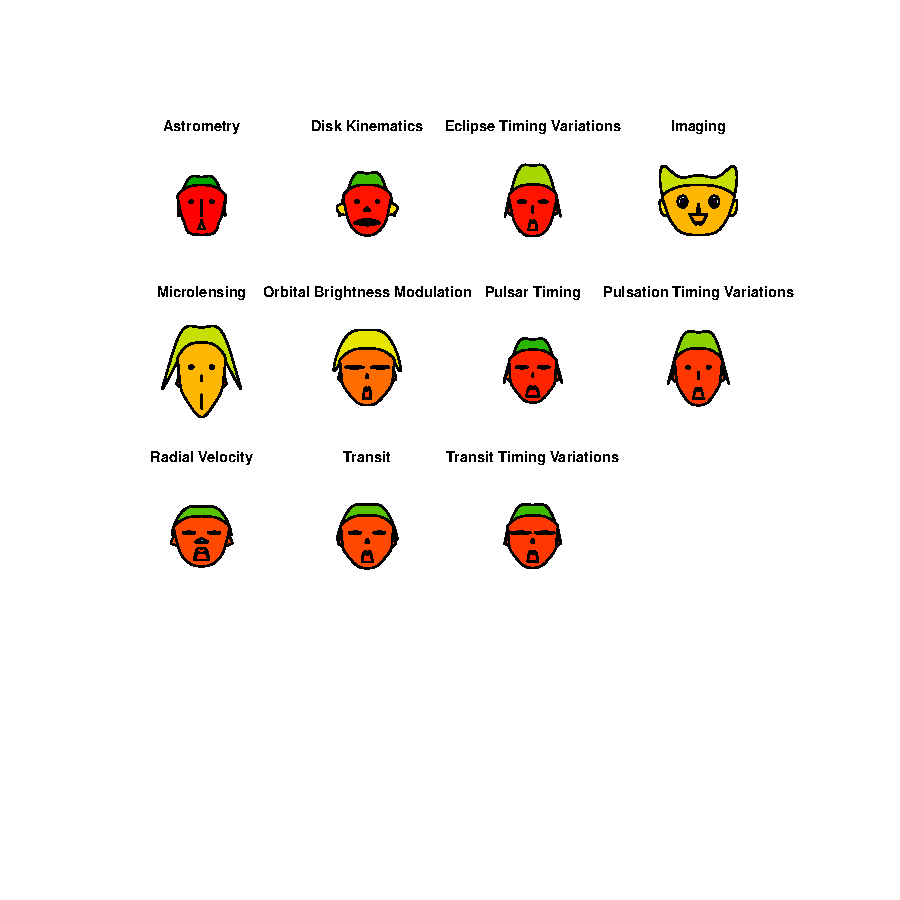
\includegraphics[width = 1.4\textwidth]{exoplanety-faces.pdf}
\vspace{-3.25in}
\end{figure}

Na Chernoffových tvářích jsou ukázány rozdíly průměrných hodnot planet mezi planetami objevenými jednotlivými metodami.

\setlength{\columnsep}{0\textwidth}
\begin{center}
\begin{multicols}{3}
\begin{minipage}{\columnwidth}
% latex table generated in R 3.5.2 by xtable 1.8-4 package
% Mon Dec  9 22:38:36 2019
\begin{tabular}{| l| l|}
  \hline
{\cellcolor[rgb]{0.85, 0.85, 0.85}{ modified.item }} & {\cellcolor[rgb]{0.85, 0.85, 0.85}{ Var }} \\ 
  \hline
height of face    & dist \\ 
   \hline
width of face     & rad \\ 
   \hline
structure of face & mass \\ 
   \hline
height of mouth   & srad \\ 
   \hline
width of mouth    & smass \\ 
   \hline
\end{tabular}\end{minipage}
\begin{minipage}{\columnwidth}
% latex table generated in R 3.5.2 by xtable 1.8-4 package
% Mon Dec  9 22:38:36 2019
\begin{tabular}{| l| l|}
  \hline
{\cellcolor[rgb]{0.85, 0.85, 0.85}{ modified.item }} & {\cellcolor[rgb]{0.85, 0.85, 0.85}{ Var }} \\ 
  \hline
smiling           & smax \\ 
   \hline
height of eyes    & per \\ 
   \hline
width of eyes     & pnum \\ 
   \hline
height of hair    & stem \\ 
   \hline
width of hair    & dist \\ 
   \hline
\end{tabular}\end{minipage}
\begin{minipage}{\columnwidth}
% latex table generated in R 3.5.2 by xtable 1.8-4 package
% Mon Dec  9 22:38:36 2019
\begin{tabular}{| l| l|}
  \hline
{\cellcolor[rgb]{0.85, 0.85, 0.85}{ modified.item }} & {\cellcolor[rgb]{0.85, 0.85, 0.85}{ Var }} \\ 
  \hline
style of hair    & rad \\ 
   \hline
height of nose   & mass \\ 
   \hline
width of nose    & srad \\ 
   \hline
width of ear     & smass \\ 
   \hline
height of ear    & smax \\ 
   \hline
\end{tabular}\end{minipage}
\end{multicols}
\end{center}
\vspace{-0.35in}
% latex table generated in R 3.5.2 by xtable 1.8-4 package
% Mon Dec  9 22:38:36 2019
\begin{table}[ht]
\centering
\begin{tabular}{| l| l|}
   \hline
\end{tabular}
\caption{Vlastnosti tváří popisující vlastnosti planet} 
\end{table}
\newpage
\section{Korelační matice}

% latex table generated in R 3.5.2 by xtable 1.8-4 package
% Mon Dec  9 22:38:36 2019
\begin{table}[ht]
\centering
\begin{tabular}{| l| l| l| l| l| l| l| l| l| l|}
  \hline
 & {\cellcolor[rgb]{0.85, 0.85, 0.85}{ dist }} & {\cellcolor[rgb]{0.85, 0.85, 0.85}{ mass }} & {\cellcolor[rgb]{0.85, 0.85, 0.85}{ rad }} & {\cellcolor[rgb]{0.85, 0.85, 0.85}{ smax }} & {\cellcolor[rgb]{0.85, 0.85, 0.85}{ per }} & {\cellcolor[rgb]{0.85, 0.85, 0.85}{ pnum }} & {\cellcolor[rgb]{0.85, 0.85, 0.85}{ smass }} & {\cellcolor[rgb]{0.85, 0.85, 0.85}{ srad }} & {\cellcolor[rgb]{0.85, 0.85, 0.85}{ stem }} \\ 
  \hline
{\cellcolor[rgb]{0.85, 0.85, 0.85}{ dist }} & {\cellcolor[rgb]{ 0 ,  1 ,  0 }{ 1 }} & {\cellcolor[rgb]{ 0.83 ,  1 ,  0.83 }{ 0.17 }} & {\cellcolor[rgb]{ 0.8 ,  1 ,  0.8 }{ 0.2 }} & {\cellcolor[rgb]{ 1 ,  0.99 ,  0.99 }{ -0.01 }} & {\cellcolor[rgb]{ 1 ,  0.96 ,  0.96 }{ -0.04 }} & {\cellcolor[rgb]{ 1 ,  0.89 ,  0.89 }{ -0.11 }} & {\cellcolor[rgb]{ 0.69 ,  1 ,  0.69 }{ 0.31 }} & {\cellcolor[rgb]{ 0.66 ,  1 ,  0.66 }{ 0.34 }} & {\cellcolor[rgb]{ 0.75 ,  1 ,  0.75 }{ 0.25 }} \\ 
   \hline
{\cellcolor[rgb]{0.85, 0.85, 0.85}{ mass }} & {\cellcolor[rgb]{ 0.83 ,  1 ,  0.83 }{ 0.17 }} & {\cellcolor[rgb]{ 0 ,  1 ,  0 }{ 1 }} & {\cellcolor[rgb]{ 0.75 ,  1 ,  0.75 }{ 0.25 }} & {\cellcolor[rgb]{ 0.84 ,  1 ,  0.84 }{ 0.16 }} & {\cellcolor[rgb]{ 0.85 ,  1 ,  0.85 }{ 0.15 }} & {\cellcolor[rgb]{ 1 ,  0.81 ,  0.81 }{ -0.19 }} & {\cellcolor[rgb]{ 0.78 ,  1 ,  0.78 }{ 0.22 }} & {\cellcolor[rgb]{ 0.84 ,  1 ,  0.84 }{ 0.16 }} & {\cellcolor[rgb]{ 0.91 ,  1 ,  0.91 }{ 0.09 }} \\ 
   \hline
{\cellcolor[rgb]{0.85, 0.85, 0.85}{ rad }} & {\cellcolor[rgb]{ 0.8 ,  1 ,  0.8 }{ 0.2 }} & {\cellcolor[rgb]{ 0.75 ,  1 ,  0.75 }{ 0.25 }} & {\cellcolor[rgb]{ 0 ,  1 ,  0 }{ 1 }} & 0 & {\cellcolor[rgb]{ 0.97 ,  1 ,  0.97 }{ 0.03 }} & {\cellcolor[rgb]{ 1 ,  0.36 ,  0.36 }{ -0.64 }} & {\cellcolor[rgb]{ 0.42 ,  1 ,  0.42 }{ 0.58 }} & {\cellcolor[rgb]{ 0.57 ,  1 ,  0.57 }{ 0.43 }} & {\cellcolor[rgb]{ 0.82 ,  1 ,  0.82 }{ 0.18 }} \\ 
   \hline
{\cellcolor[rgb]{0.85, 0.85, 0.85}{ smax }} & {\cellcolor[rgb]{ 1 ,  0.99 ,  0.99 }{ -0.01 }} & {\cellcolor[rgb]{ 0.84 ,  1 ,  0.84 }{ 0.16 }} & 0 & {\cellcolor[rgb]{ 0 ,  1 ,  0 }{ 1 }} & {\cellcolor[rgb]{ 0.02 ,  1 ,  0.02 }{ 0.98 }} & {\cellcolor[rgb]{ 0.97 ,  1 ,  0.97 }{ 0.03 }} & {\cellcolor[rgb]{ 1 ,  0.95 ,  0.95 }{ -0.05 }} & {\cellcolor[rgb]{ 0.96 ,  1 ,  0.96 }{ 0.04 }} & {\cellcolor[rgb]{ 1 ,  0.95 ,  0.95 }{ -0.05 }} \\ 
   \hline
{\cellcolor[rgb]{0.85, 0.85, 0.85}{ per }} & {\cellcolor[rgb]{ 1 ,  0.96 ,  0.96 }{ -0.04 }} & {\cellcolor[rgb]{ 0.85 ,  1 ,  0.85 }{ 0.15 }} & {\cellcolor[rgb]{ 0.97 ,  1 ,  0.97 }{ 0.03 }} & {\cellcolor[rgb]{ 0.02 ,  1 ,  0.02 }{ 0.98 }} & {\cellcolor[rgb]{ 0 ,  1 ,  0 }{ 1 }} & {\cellcolor[rgb]{ 0.99 ,  1 ,  0.99 }{ 0.01 }} & {\cellcolor[rgb]{ 1 ,  0.95 ,  0.95 }{ -0.05 }} & {\cellcolor[rgb]{ 0.98 ,  1 ,  0.98 }{ 0.02 }} & {\cellcolor[rgb]{ 1 ,  0.95 ,  0.95 }{ -0.05 }} \\ 
   \hline
{\cellcolor[rgb]{0.85, 0.85, 0.85}{ pnum }} & {\cellcolor[rgb]{ 1 ,  0.89 ,  0.89 }{ -0.11 }} & {\cellcolor[rgb]{ 1 ,  0.81 ,  0.81 }{ -0.19 }} & {\cellcolor[rgb]{ 1 ,  0.36 ,  0.36 }{ -0.64 }} & {\cellcolor[rgb]{ 0.97 ,  1 ,  0.97 }{ 0.03 }} & {\cellcolor[rgb]{ 0.99 ,  1 ,  0.99 }{ 0.01 }} & {\cellcolor[rgb]{ 0 ,  1 ,  0 }{ 1 }} & {\cellcolor[rgb]{ 1 ,  0.64 ,  0.64 }{ -0.36 }} & {\cellcolor[rgb]{ 1 ,  0.76 ,  0.76 }{ -0.24 }} & {\cellcolor[rgb]{ 1 ,  0.82 ,  0.82 }{ -0.18 }} \\ 
   \hline
{\cellcolor[rgb]{0.85, 0.85, 0.85}{ smass }} & {\cellcolor[rgb]{ 0.69 ,  1 ,  0.69 }{ 0.31 }} & {\cellcolor[rgb]{ 0.78 ,  1 ,  0.78 }{ 0.22 }} & {\cellcolor[rgb]{ 0.42 ,  1 ,  0.42 }{ 0.58 }} & {\cellcolor[rgb]{ 1 ,  0.95 ,  0.95 }{ -0.05 }} & {\cellcolor[rgb]{ 1 ,  0.95 ,  0.95 }{ -0.05 }} & {\cellcolor[rgb]{ 1 ,  0.64 ,  0.64 }{ -0.36 }} & {\cellcolor[rgb]{ 0 ,  1 ,  0 }{ 1 }} & {\cellcolor[rgb]{ 0.28 ,  1 ,  0.28 }{ 0.72 }} & {\cellcolor[rgb]{ 0.64 ,  1 ,  0.64 }{ 0.36 }} \\ 
   \hline
{\cellcolor[rgb]{0.85, 0.85, 0.85}{ srad }} & {\cellcolor[rgb]{ 0.66 ,  1 ,  0.66 }{ 0.34 }} & {\cellcolor[rgb]{ 0.84 ,  1 ,  0.84 }{ 0.16 }} & {\cellcolor[rgb]{ 0.57 ,  1 ,  0.57 }{ 0.43 }} & {\cellcolor[rgb]{ 0.96 ,  1 ,  0.96 }{ 0.04 }} & {\cellcolor[rgb]{ 0.98 ,  1 ,  0.98 }{ 0.02 }} & {\cellcolor[rgb]{ 1 ,  0.76 ,  0.76 }{ -0.24 }} & {\cellcolor[rgb]{ 0.28 ,  1 ,  0.28 }{ 0.72 }} & {\cellcolor[rgb]{ 0 ,  1 ,  0 }{ 1 }} & {\cellcolor[rgb]{ 0.83 ,  1 ,  0.83 }{ 0.17 }} \\ 
   \hline
{\cellcolor[rgb]{0.85, 0.85, 0.85}{ stem }} & {\cellcolor[rgb]{ 0.75 ,  1 ,  0.75 }{ 0.25 }} & {\cellcolor[rgb]{ 0.91 ,  1 ,  0.91 }{ 0.09 }} & {\cellcolor[rgb]{ 0.82 ,  1 ,  0.82 }{ 0.18 }} & {\cellcolor[rgb]{ 1 ,  0.95 ,  0.95 }{ -0.05 }} & {\cellcolor[rgb]{ 1 ,  0.95 ,  0.95 }{ -0.05 }} & {\cellcolor[rgb]{ 1 ,  0.82 ,  0.82 }{ -0.18 }} & {\cellcolor[rgb]{ 0.64 ,  1 ,  0.64 }{ 0.36 }} & {\cellcolor[rgb]{ 0.83 ,  1 ,  0.83 }{ 0.17 }} & {\cellcolor[rgb]{ 0 ,  1 ,  0 }{ 1 }} \\ 
   \hline
\end{tabular}
\caption{Korelační matice} 
\end{table}
V~korelační matici lze vidět lineární závislost mezi velkou poloosou a~dobou oběhu planety, která vychází z~Keplerových zákonů. Slabá záporná korelace je i~mezi počtem planet a~poloměrem planety. Čím větší planeta je, tím spíše bude v~soustavě méně planet.

Velice slabá korelace (0,58) je viditelná mezi hmotností hvězdy a~poloměrem planety. U~hmotnějších hvězd byly častěji pozorovány větší planety. Naopak vzdálenost planety od Země nezávisí na žádném jiném údaji -- planety všech možných vlastností jsou objevovány v různých vzdálenostech od Země.

\section{Chí-kvadrát test}


Do kontingenční tabulky byla umístěna četnost planet v~různých velikostních kategoriích v~závislosti na periodě oběhu kolem hvězdy. Kvůli nedostatku objevených ledových planet se poslední sloupec nebude promítat do testu nezávislosti.

\begin{figure}[!htb]
  \centering
  \begin{subfigure}[b]{0.5\textwidth}
% latex table generated in R 3.5.2 by xtable 1.8-4 package
% Mon Dec  9 22:38:36 2019
\begin{tabular}{| l| l| l| l|}
  \hline
 & {\cellcolor[rgb]{0.85, 0.85, 0.85}{ Lava }} & {\cellcolor[rgb]{0.85, 0.85, 0.85}{ Hot }} & {\cellcolor[rgb]{0.85, 0.85, 0.85}{ Normal }} \\ 
  \hline
{\cellcolor[rgb]{0.85, 0.85, 0.85}{ Mercurian }} & {\cellcolor[rgb]{ 0.985641025641026 ,  1 ,  0.985641025641026 }{ 14 }} & {\cellcolor[rgb]{ 0.988717948717949 ,  1 ,  0.988717948717949 }{ 11 }} & 0 \\ 
   \hline
{\cellcolor[rgb]{0.85, 0.85, 0.85}{ Earth }} & {\cellcolor[rgb]{ 0.48 ,  1 ,  0.48 }{ 507 }} & {\cellcolor[rgb]{ 0.313846153846154 ,  1 ,  0.313846153846154 }{ 669 }} & {\cellcolor[rgb]{ 0.950769230769231 ,  1 ,  0.950769230769231 }{ 48 }} \\ 
   \hline
{\cellcolor[rgb]{0.85, 0.85, 0.85}{ Neptunian }} & {\cellcolor[rgb]{ 0.863589743589744 ,  1 ,  0.863589743589744 }{ 133 }} & {\cellcolor[rgb]{ 0 ,  1 ,  0 }{ 975 }} & {\cellcolor[rgb]{ 0.794871794871795 ,  1 ,  0.794871794871795 }{ 200 }} \\ 
   \hline
{\cellcolor[rgb]{0.85, 0.85, 0.85}{ Jovian }} & {\cellcolor[rgb]{ 0.602051282051282 ,  1 ,  0.602051282051282 }{ 388 }} & {\cellcolor[rgb]{ 0.866666666666667 ,  1 ,  0.866666666666667 }{ 130 }} & {\cellcolor[rgb]{ 0.942564102564103 ,  1 ,  0.942564102564103 }{ 56 }} \\ 
   \hline
\end{tabular}  \end{subfigure}
  \begin{subfigure}[b]{0.2\textwidth}
% latex table generated in R 3.5.2 by xtable 1.8-4 package
% Mon Dec  9 22:38:36 2019
\begin{tabular}{| l|}
  \hline
{\cellcolor[rgb]{0.85, 0.85, 0.85}{ Cold }} \\ 
  \hline
0 \\ 
   \hline
0 \\ 
   \hline
5 \\ 
   \hline
11 \\ 
   \hline
\end{tabular}  \end{subfigure}
  \vspace{-1cm}
\end{figure}
% latex table generated in R 3.5.2 by xtable 1.8-4 package
% Mon Dec  9 22:38:36 2019
\begin{table}[ht]
\centering
\begin{tabular}{| l| l|}
   \hline
\end{tabular}
\caption{Četnost planet dle velikosti a periody oběhu hvězdy} 
\end{table}
\begin{itemize}
  \item H\textsubscript{0}:~Vzdálenost planet od mateřské hvězdy nezávisí na jejich velikosti.
  \item H\textsubscript{1}:~Existuje spojitost mezi vzdáleností planety od hvězdy a~její velikostí.
\end{itemize}

\begin{Schunk}
\begin{Soutput}
	Pearson's Chi-squared test

data:  size.vs.period[, 1:3]
X-squared = 719.24, df = 6, p-value < 2.2e-16
\end{Soutput}
\end{Schunk}

Protože p-value je dostatečně malá, velikost planety a její perioda oběhu jsou závislé proměnné.

\section{T-test}

Cílem t-testu je demonstrovat na příkladu závěr chí-kvadrát testu v~předchozí kapitole~--~velikost planety a~perioda oběhu kolem hvězdy jsou závislé proměnné. Pro tento účel byl proveden náhodný výběr o~velikosti 1~/~10 z~velikostních kategorií planet Neptunian a~Earth. T-test testuje doby periody planet v těchto náhodných výběrech.

\begin{Schunk}
\begin{Soutput}
	Two Sample t-test

data:  earths$per and neptunians$per
t = -3.9297, df = 251, p-value = 0.00011
alternative hypothesis: true difference in means is not equal to 0
95 percent confidence interval:
 -33.19149 -11.02941
sample estimates:
mean of x mean of y 
 11.86790  33.97836 
\end{Soutput}
\end{Schunk}

Protože p-value je menší než~0,05, můžeme nulovou hypotézu na 95\% hladině významnosti zamítnout a~říct, že střední hodnota period oběhů planet ve skupinách Earth a~Neptunian není stejná. V konfidenčním intervalu je uvedeno, že střední hodnota periody oběhu planet typu Earth je o~několik jednotek až desítek (dní) menší, než u~planet ze skupiny Neptunian.

\section{QQplot}

V kapitole 2.10 bylo řečeno, že nejvíce objevených exoplanet obíhá kolem hvězd s~podobnou teplotou jako naše Slunce. Do QQ grafu bude proto zanesena právě povrchová teplota hvězd, u níž se bude zjišťovat, zda vyhovuje normálnímu rozdělení.

\begin{figure}[!htb]
  \centering
  \begin{subfigure}[b]{0.7\textwidth}
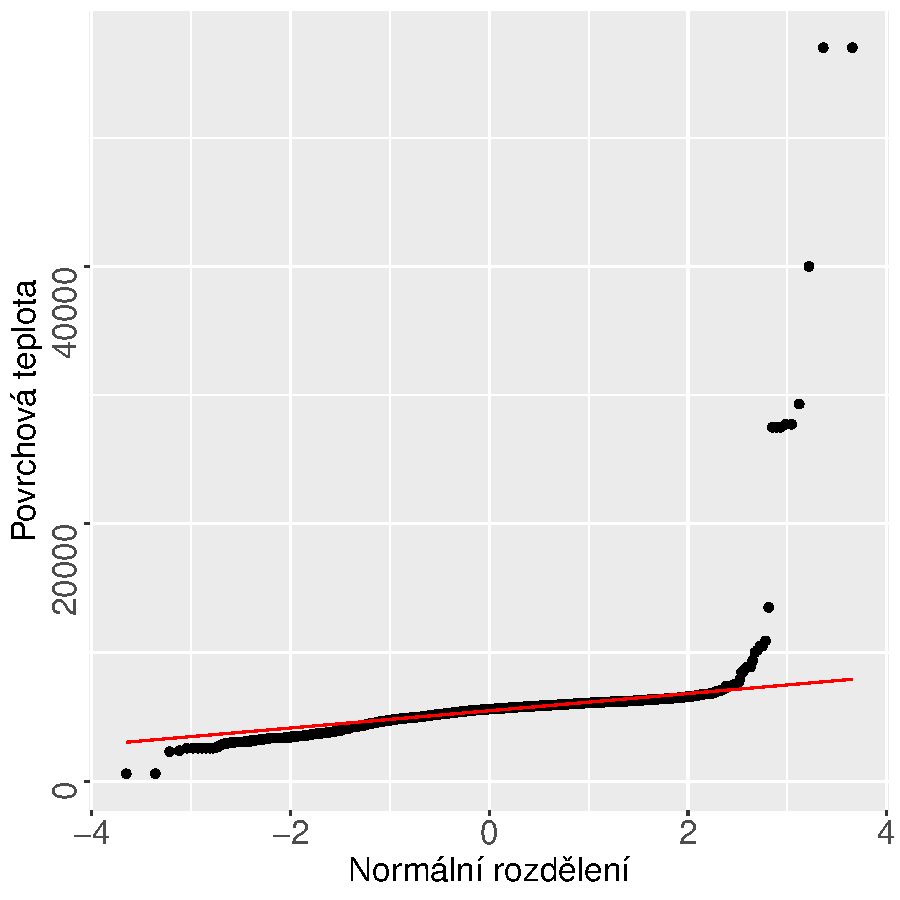
\includegraphics{exoplanety-028}
  \end{subfigure}
\end{figure}

Většina bodů leží na požadované přímce, a~proto lze říci, že rozdělení teplot je blízké normálnímu rozdělení. Výjimkou jsou extrémy, které se od normálního rozdělení vzdalují.

\section{Analýza rozptylu}

\begin{center}
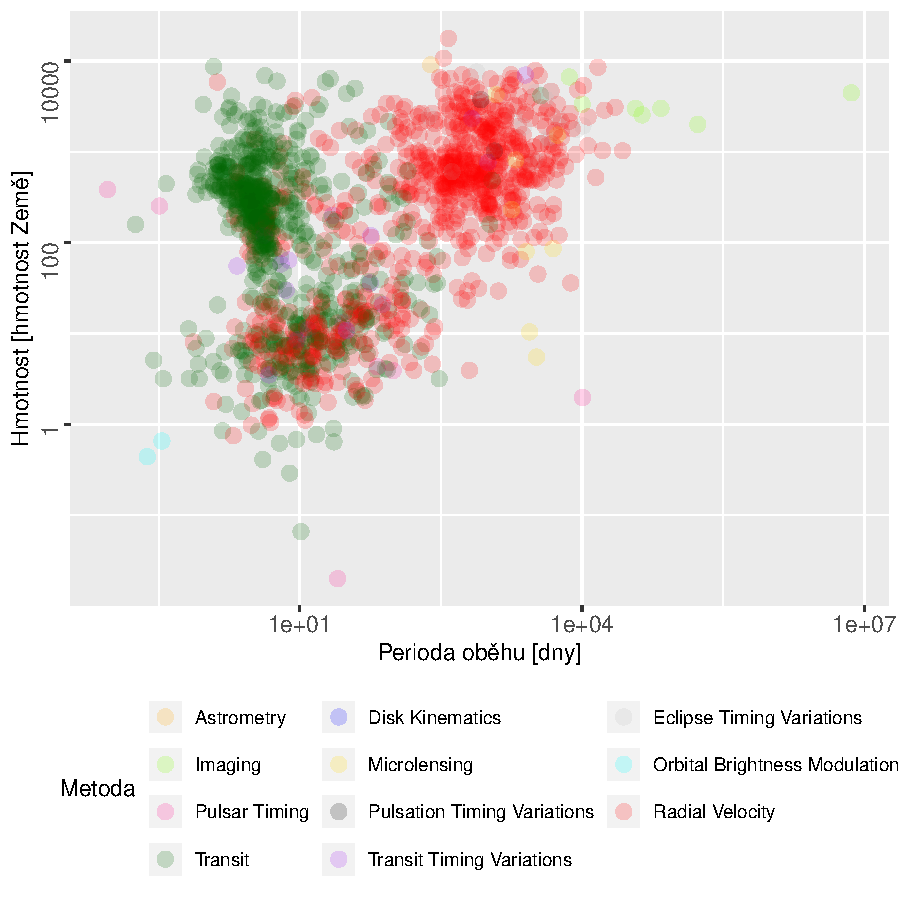
\includegraphics{exoplanety-029}
\end{center}

Graf výše ukazuje rozdílné hmotnosti a periody planet při rozdílných metodách objevení. Hmotné hvězdy blízko své hvězdy byly objevovány převážně metodou Transit, kdežto hmotné hvězdy daleko od své hvězdy metodou Radial Velocity.

\begin{Schunk}
\begin{Soutput}
                   Df    Sum Sq   Mean Sq  F value   Pr(>F)    
stype               3 1.562e+08 5.207e+07   10.415 8.12e-07 ***
meth                4 2.116e+10 5.289e+09 1058.009  < 2e-16 ***
dtype               1 1.438e+05 1.438e+05    0.029    0.865    
stype:meth          4 3.371e+03 8.430e+02    0.000    1.000    
stype:dtype         3 2.319e+05 7.730e+04    0.015    0.997    
meth:dtype          1 4.200e+01 4.200e+01    0.000    0.998    
stype:meth:dtype    1 2.750e+02 2.750e+02    0.000    0.994    
Residuals        3128 1.564e+10 4.999e+06                      
---
Signif. codes:  0 ‘***’ 0.001 ‘**’ 0.01 ‘*’ 0.05 ‘.’ 0.1 ‘ ’ 1
958 observations deleted due to missingness
\end{Soutput}
\end{Schunk}

Ve výsledcích analýzy rozptylu je uvedeno, že na dobu periody skutečně má vliv metoda objevení (meth) i velikost (stype). Naproti tomu vzdálenost od Země (dtype) nikoliv.

\newpage

\section{Regrese}

Cílem regrese je určit, zda počet publikací objevů exoplanet v průběhu posledních let klesá nebo stoupá.

\begin{center}
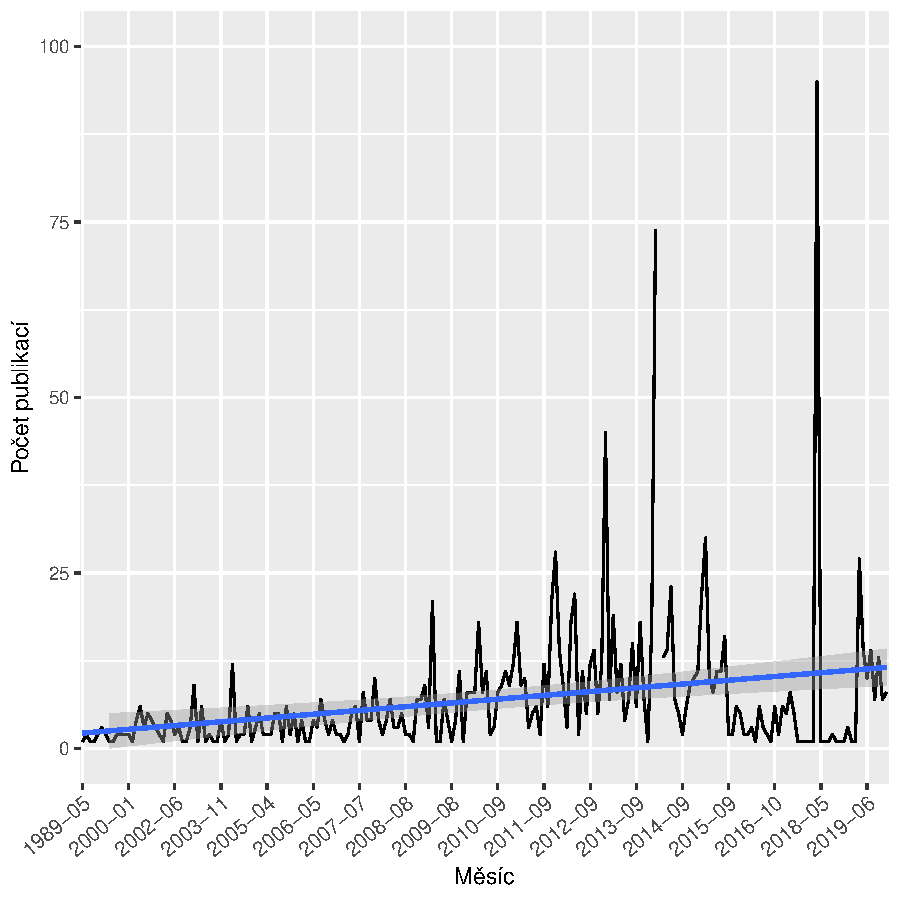
\includegraphics{exoplanety-031}
\end{center}

Měsíční počet publikací exoplanet stále stoupá. V~grafu je vyznačen i~95\% interval spolehlivosti.

\newpage

\section{Boxplot}

V závěrečné kapitole budou na boxplotu zobrazeny statistiky poloměrů planet v~závislosti na spektrální třídě hvězdy, kolem které obíhají.

\begin{center}
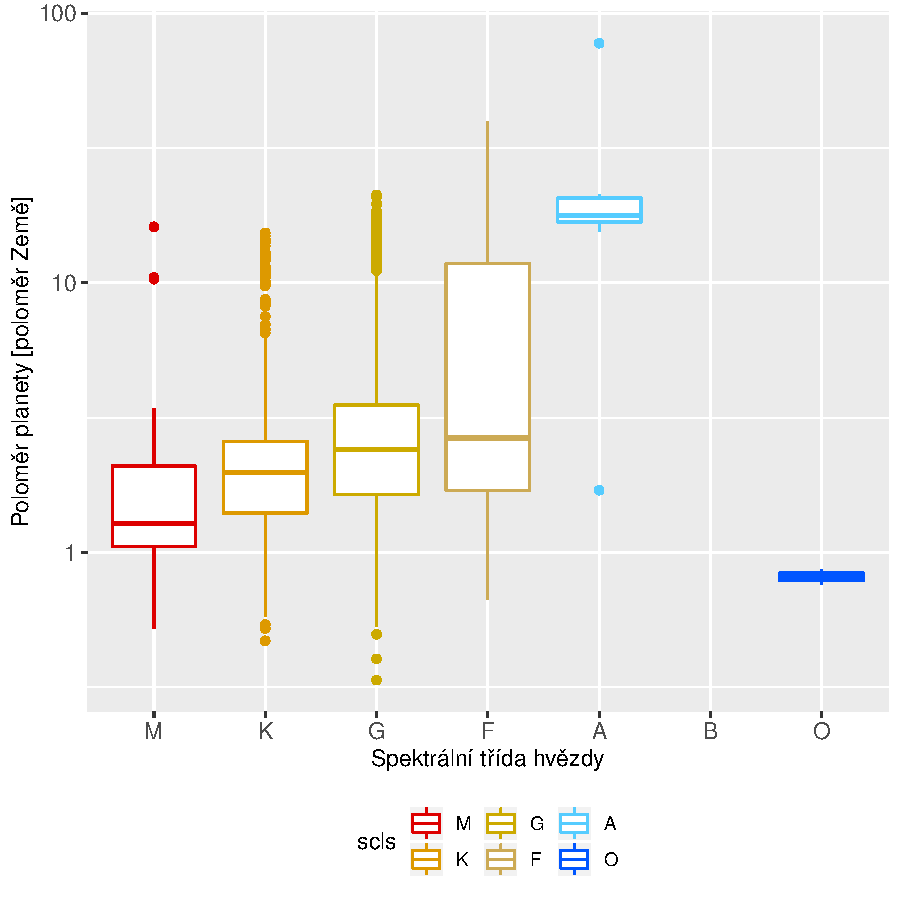
\includegraphics{exoplanety-032}
\end{center}

Největší planety obíhají kolem modrobílých hvězd (třída A). Nejmenší objevená planeta obíhá kolem žluté hvězdy (třída G). Kolem hvězd třídy B byla objevena pouze jedna planeta, a~proto není box pro tuto skupinu zobrazen.

\end{document}
